\documentclass[letterpaper, 12pt]{article}
\usepackage{cmjStyle}
\usepackage{natbib}
\usepackage{hyperref}
\bibpunct{(}{)}{;}{a}{}{,}
\doublespacing
\raggedright
\setlength{\parskip}{2ex}
\parindent 24pt
\urlstyle{same}
\setcounter{secnumdepth}{-1}

%\usepackage{endfloat}

\begin{document}

 {\cmjTitle Vivace: A Collaborative Live Coding Language}

%% %author - name
{\cmjAuthor Vilson Vieira, Guilherme Lunhani, Geraldo Magela de Castro
  Rocha Junior, Caleb Mascarenhas Luporini, Daniel Penalva, Ricardo
  Fabbri, Renato Fabbri
%% %author - address
\newline
\begin{cmjAuthorAddress}
  Instituto de F\'{i}sica de S\~{a}o Carlos\\
  Universidade de S\~{a}o Paulo\\
  Avenida Trabalhador S\~{a}o-carlense, 400\\
  Parque Arnold Schimidt\\
  S\~{a}o Carlos, S\~{a}o Paulo 13566-590 Brazil\\

  vilson@void.cc, gcravista@gmail.com, gera.sp@gmail.com,
  calebml@gmail.com, dkajah@gmail.com, rfabbri@gmail.com,
  renato.fabbri@gmail.com
\end{cmjAuthorAddress}

\vspace*{24pt}

%{\cmjAuthorPhone << AUTHOR TELEPHONE (not for publication): +55 16 8108 7007 >>}
\section*{Abstract}

This paper describes the principles and the design of Vivace, a live
coding language and environment built with Web technologies to be
executed, ideally, in any ordinary browser. It starts by reviewing
what motivated and inspired the creation of the language, in the
context of actual performances. That leads to specifications of the
language and how it is parsed and then executed using the recently
created real-time Web Audio API. A brief discussion is presented on
why the Web is an environment of interest to collaborative live coding
and how it affects the performances. This work concludes by describing
how Vivace has motivated the creation of ``freak coding'', a live
coding sub-genre.

\section*{} % Introdução, sem título.

In November of 2011, a live coding trio called
\textit{FooBarBaz}~\citep{foobarbaz} unleashed its first presentation
for a wide audience. Its performers were using two instances of
ChucK~\citep{wang2003chuck} and a dedicated mixing Puredata + Analog
Mixer instance~\footnote{Pictures of the presentation available at
  \url{http://www.flickr.com/photos/festivalcontato/6436260557}}. Live
coding has been gaining world wide popularity~\citep{nilson2007live,
  collins2003live, brown2007a, collins2011live}, while remaining quite
untouched in Brazil. To the best of our knowledge, that presentation
was the first live coding performance in our country -- almost 5,000
attendees were in the audience where code was used on-the-fly to
create the music they were listening. At the same time, two live
coding desktop work-spaces were projected on big screens to the
public, following the principles from the \textsc{toplap}
manifesto~\citep{ward2004live}.

During the performance, the trio used ChucK in an unconventional
way. Instead of writing loops and conditionals, one of the live coders
manipulated parameters of audio files by editing lists of numerical
values together with mnemonic operations like retrograde and
transposition.  The other live coder focused on more fluid lines with
large sounds having evolving characteristics; this contributed with
larger musical arcs.  Audio mixing with Puredata was carried out by
the third performer literally using handwaving gestures tracked by a
camera and our custom-designed color detection algorithms. Live coders
used code templates quick-inserted by programmer's text editors (Vi
and Emacs). Other visual resources the performers focused on were:
Unix ``cowsay'' generated phrases on individual terminals and animated
bouncing balls -- stimulating the audience to imitate Rapid Eyes
Movements (REM). These artifacts -- code, ``cowsay'' phrases, moving
REM-like points of reference, all projected in big screens to the
public -- were incorporated as good practices during the live coding
performance.

Based on the aforementioned elements, a new language was designed:
Vivace~\footnote{Live demonstrations of Vivace are on-line at
    \url{http://void.cc/freakcoding} and~\url{http://void.cc/cranio},
    ready to be used by everyone using
  Google Chrome or Apple Safari.}~\citep{Vivace}.  To avoid software
configuration and to make it easy to share the session -- and the
system itself -- with everyone, the Web was chosen as the running
environment for Vivace. On every new session performed using Vivace,
new principles were added into the language and, at the same time,
into our artistic behavior.

In summary, this paper has a circular structure: it describes how
actual performances motivated the language and how the language itself
influenced the creation of a live coding sub-genre that is being
developed by many hands, called ``freak coding'' by its
manifesto~\citep{freak}, other written resources, and in spoken
instances.

\parskip 18pt

\section{Additional motivation \& inspiration: arrange the room, the code is dirty}

Vivace is inspired by various live coding languages. The syntax of
Vivace, as shown in Figure~\ref{fig:vivace}, borrows elements from ixi
lang~\citep{magnusson2011ixi} such as the use of sequences to control
audio parameters in real time. ABT~\citep{fabbri} and
FIGGUS~\citep{fabbri2} were tightly relevant to the development of
Vivace as well and we are planning to rewrite some of their components
-- originally in Python -- inside Vivace. ChucK suggested chained unit
generators specified by the $=>$ operator, mimicking the object
connections in visual programming languages like
Puredata. Fluxus~\citep{fluxus} was also inspirational for the Vivace
environment where the code is shown on top of the video frames.

\begin{figure}[htpb]
  \begin{center}
    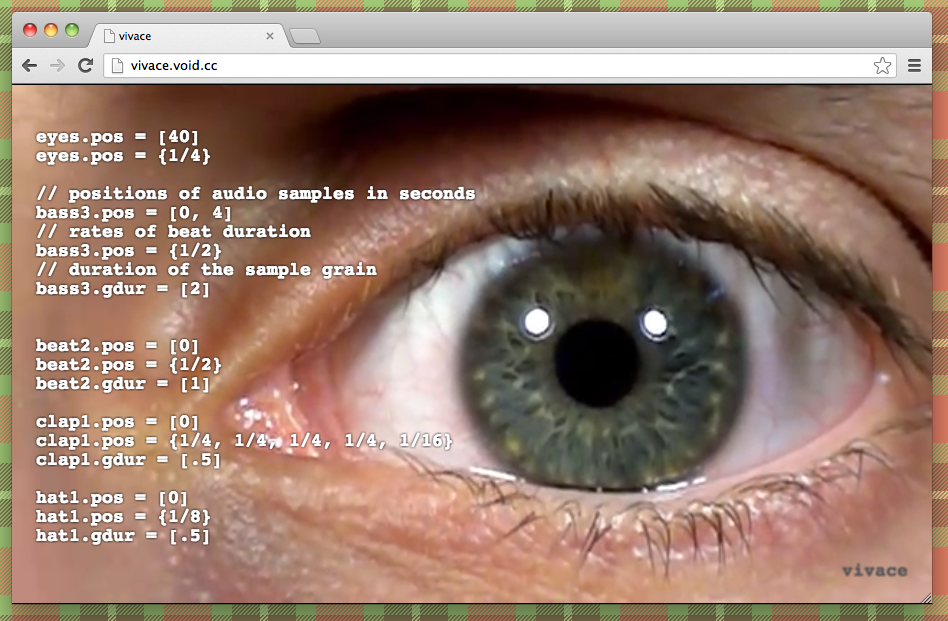
\includegraphics[scale=.4]{img/fig_vivace.png}
    \caption{The Vivace environment.}
    \label{fig:vivace}
  \end{center}
\end{figure}

After the creation of Audio Data API~\citep{audiodata} and the most
recent Web Audio API~\citep{webaudio} -- enabling real time audio
processing inside Web browsers -- a collection of audio Web
applications started to emerge. The same holds for live coding
languages and systems.  Thus, in addition to the \textit{desktop
  languages} pointed above, Vivace was also inspired by recent Web
live coding languages and is part of this \textit{family} of Web
applications together with Gibber~\citep{gibber},
livecoder~\citep{livecoder}, livecoding.io~\citep{livecodingio} and
livecodelab~\citep{livecodelab}, to note some of them.

A remarkable difference between Vivace and other languages or
environments in the same family is the element of
collaborativity. Vivace was built to enable writing code with many
hands at the same time, as with the now popular ``e-pads'' or
collaborative real-time text editors~\footnote{Etherpad on:
  \url{http://etherpad.org}.}, a feature which is naturally
implementable on the Web. Another difference is the unconcern to be a
Turing-complete language. This made the design of Vivace more flexible
and closer to the musical process rather than the computing process (a
characteristic perceived in ixi lang as well). Vivace tries to place
itself between the precision of code and the flexibility of artistic
expression.

\section{The language (specification) we all speak}

Vivace, as a language~\footnote{The complete specification can be
  found at
  \url{https://github.com/automata/vivace/wiki/Language-spec}.}, is a
collaborative live coding language with use of extremely simple
syntax, mnemonic operations, easy audio mixing, template editing and
audio parameters automation. The use of shared code, sounds and images
leads to a more complex scenario, thus increasing the possibility of
inconsistency of compiled code as well as actions for artistic
result. This enhances the fit of specific language syntax.

Vivace is not an imperative language. Instead of routines and
procedures to control audio attributes, it uses definitions related
with musical scores and the \emph{track paradigm} common on music
production software. It is natural to musicians (and, as we
experienced during performances, also to non-musicians) to understand
a sequence of notes, or audio parameters, repeating over and over
again, than a for-loop and if-chains. In this way, Vivace is a
declarative, domain specific language, based on the following
principles:

\begin{itemize}
  
\item Names are literals like $foo$, $bar$, $baz$ and are defined as
  the user wants.
\item Music is made by voices (instruments).
\item Voices have name, timbre and parameters changing along time.
\item The language should be simple. ``Freak coders'', with a
  dedicated section below, only define some properties with a set of
  values (i.e. arrays, dictionaries) making it possible to generate
  sequences, even using list comprehension.
\item Mnemonic musical operations (reverse, inverse, transpose) on
  properties by use of syntax sugar: few chars, big results.
\item Timbre are signals made by chains of audio generators and
  filters or video files as described below.
\item Parameters are musical notes, amplitudes, oscillator
  frequencies, delay time and so on.
\item Parameters change their values at specific times and for certain
  durations.
\end{itemize}

Here is a ``Hello, World!'' Vivace code:

\begin{Verbatim}[fontfamily=courier, xleftmargin=\parindent]
# foo is a simple audio sample, oscillator or video file
foo.src = youtube('http://www.youtube.com/watch?v=XXX')
# defining the video positions (in seconds) to be played
foo.pos = [10, 20, 35]
# the durations (as time ratios) to play each position
foo.cdur = [1/2, 1/4, 1/8, 1/16, 1]
\end{Verbatim}

A voice is defined as \textit{foo} and its parameters are specified
using the \textit{dot} operator. Every parameter changes over time as
the values written as numerical sequences, surrounded by brackets. A
special sequence exists to every parameter. This is essentially all of
the Vivace syntax.

There are extra semantics to operate on the sequences. Every sequence
accepts operators: mnemonic commands used to reverse, transpose and
even replace elements of the sequence based on list
comprehensions. Those operations are common in music composition and
having them as mnemonics makes typing fast and handy for live
coding. The next listing presents the standard operators:

\begin{Verbatim}[fontfamily=courier, xleftmargin=\parindent]
# we can use operators
foo.pos = [1, 2, 3] reverse        # result is [3, 2, 1]
foo.pos = [1, 2, 3] inverse        # result is [1, 0, -1]
foo.pos = [1, 2, 3] transpose +2   # result is [3, 4, 5]

# and even list comprehension
foo.pos = [1/i+1 for i in [1, 2, 3]] 
# result is [2, 3, 4]

# or combine both
foo.pos = [1/i+1 for i in [1, 2, 3]] reverse 
# result is [4, 3, 2] as expected
\end{Verbatim}

Vivace is written in JavaScript to take advantage of Web technologies.
To parse Vivace, Jison~\citep{jison} comes handy, a JavaScript
library that clones Flex and Bison functionality as lexer and
parser. This flexibility to parse and execute new languages as
JavaScript inside every browser opens a remarkable opportunity to
experiment with new syntax and semantics for live coding. To make the
Vivace editor collaborative we used ShareJS~\citep{sharejs} which make
Web applications content live concurrent. In this way it was possible
to share Vivace code with any user accessing a common
URL. Furthermore, considering the tradition of UI design and
development on the Web thanks to HTML and CSS, one can experiment
those new languages with fast prototyped UI -- a requisite already
addressed by live coding languages~\citep{mclean2010visualisation,
  magnusson2011algorithms} like Texture~\citep{mclean2011texture},
Al-Jazari and Betablocker. Along these advantages, it is important to
note: every live coding language built on the Web runs everywhere a
browser is installed. No firewall chain to bypass for OSC, no software
installation and configuration, no dependencies, people just need to
type an URL.

\section{Vivace audio and video engine}

Before the Web Audio API, the only way to create sound in web pages
was using plug-ins. Recently, the Web Audio API enabled real time
audio processing on Web browsers~\footnote{At the time this paper was
  written, only Google Chrome and Apple Safari supported the
  API. Mozilla is working to have it running on Firefox as
  well.}. Every functionality is implemented as native code (in C++
and Assembly when appropriate) to guarantee maximum performance. The
API is based on a convenient and familiar paradigm: audio unit
graphs. Web Audio specifies a collection of nodes (\emph{AudioNode}
objects) and routines to connect and disconnect them. While
manipulating those nodes we can create a large number of audio
applications: synthesizers, filters, analyzers, mixers and even real
time audio engines to live coding. This motivated basic explorations
of multichannel expansion, filtering and audio effects, controlling an
integrated Web audio system.

Every voice in Vivace is represented as a default audio chain such as
the one shown in Figure~\ref{fig:chain}. All audio unit parameters
within this chain (e.g.\ pitch, reverb time, high, medium and low
channel levels, panner values and gain) can be manipulated editing the
code or by sliders on a GUI (Figure ~\ref{fig:ui}). This kind of
interface is more familiar to musicians, resembling a real mixer, and
enables an adequate treatment of voice timbre and spatialization of
the sound sources by means of parameters like level of stereophonic
channels L and R, quality, central frequency and gain of a 3-band
equalization filter, and reverb time control.

\begin{figure}[htpb]
  \begin{center}
    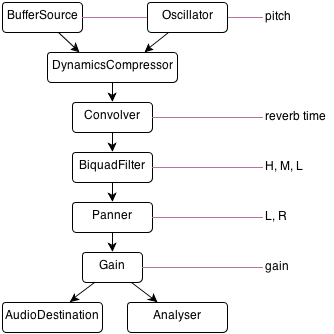
\includegraphics[scale=.5]{img/fig_chain.png}
    \caption{Standard audio unit chains as Web Audio API objects for
      each Vivace voice.}
    \label{fig:chain}
  \end{center}
\end{figure}

\begin{figure}[htpb]
  \begin{center}
    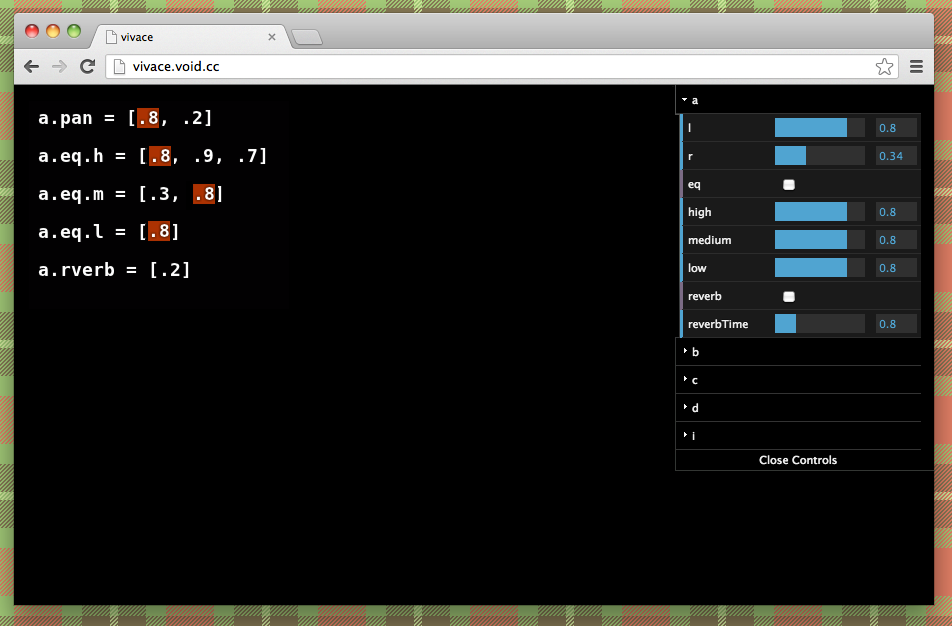
\includegraphics[scale=.4]{img/fig_ui.png}
    \caption{Every audio unit parameter can be manipulated by code or
      using the UI.}
    \label{fig:ui}
  \end{center}
\end{figure}

Vivace supports every audio unit implemented by Web Audio API. It is
possible to load audio files or synthesize in real time using
wave-table oscillators. The default audio chain of each voice can be
modified at any time while it is running. It is interesting to note
the presence of an ``Analyzer'' inside the default chain. It uses FFT
(natively implemented) to expose energies and frequencies, enabling
the use of those values to animate videos and render graphical forms
inside Vivace.

Along with audio, Vivace supports video files. It is possible to
upload files or use YouTube URLs. Videos are treated the same way as
buffer sources or oscillators, i.e.\ as voices, and can be manipulated
on real time, making Vivace a live cinema or a VJing tool.

\section{Into the wild: the rise of freak coding makes it collaborative}

Vivace as a tool enables interaction while everyone could use their
own creativity. The interaction is not mediated by a common score, but
by a mutual desire to create a composition in real time. In this
context is born the \emph{freak coder} (Figure~\ref{fig:freakcoder}):
someone that adds his individuality up to others aiming to transform
the computer into an instrument of artistic fruition without
restricting to himself the control of the machine but inviting
everyone to join him in the same activity. A freak coder decides what
he is going to do and amplifies his own comprehension of the computer
capacity as an instrument. By using simple rules, Vivace enables the
emergence of the performance and makes it a kind of a collective game,
where the rules, being visible to everyone, eases audience and
specialists alike to join in.

\begin{figure}[htpb]
  \begin{center}
    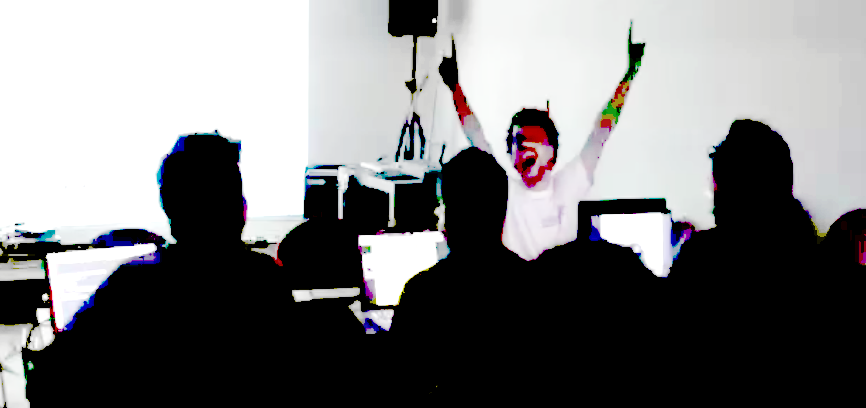
\includegraphics[scale=.4]{img/fig_freakcoder.png}
    \caption{Freak coder: a live coder who, together with others, uses
      popular and freak media to gain audience attention to the shared
      code.}
    \label{fig:freakcoder}
  \end{center}
\end{figure}

Live coding becomes a natural path to the type of use and
technological development in which freak coders are involved, in
confluence with the understanding that technology should never be
treated as a dogma or kept in secret. Live coding is seen as a
behavioral de-alienation of a digital artist. Not only the code is
displayed and manipulated, but the computer screen and potentially any
interaction between the performance and the computer. The triad
performer, code and audience characterizes the performance as live
coding.  This comprehension was possible after a presentation by
labMacambira.sourceforge.net at the $9^{th}$ edition of AVAV
(\textit{\'{A}udioVisual Ao Vivo} or Live Audiovisual), an event where
artists who are experimenting audio and video in real time come
together to show their works. In this presentation, the authors Caleb
Luporini and Gera Rocha started without Renato Fabbri and Vilson
Vieira, as they were on their way to the presentation, traveling from
another city. Upon arrival, they both turned their laptops on and
started taking part on the performance in such a way that no
embarrassment or rupture was brought into the event.  It is important
to state that no previous rehearsal had taken place between
Mr. Luporini and Mr. Rocha.\footnote{Videos were selected beforehand
  by Mr. Luporini alone without knowledge of the other performers.} In
the 30 minutes-long performance, the audience started to take guidance
from messages given on the performance big screen and actually edited
Vivace code that was being played together with the starting four
performers.

Another artifact noted on the presentation was the emergence, in a
formal environment~\footnote{The four performers were in a light-less
  room, three of them facing the big screen and the other one facing
  the public.}, of a collective euphoria fertilized by a man-machine
interaction. It is the performer's posture that takes a spectator to
an experience of a non-spectator and to take part on a highly
technological activity as something playful and possible to be
assimilated.  During the entire presentation, all
labMacambira.sourceforge.net members were cheerful and established a
relation of lightness and brotherhood with the audience.  Spectators
were being constantly invited by the posture of
labMacambira.sourceforge.net members to interact with what was being
proposed.  This interplay between the four elements therein present --
performers, computer, Vivace and audience -- was able to create an
environment of collaboration and liberty as generators of playfulness
and technical knowledge unheard of, at least in Brazilian live coding
terms. This is the ``facilitator'' that emerged and received the name
\emph{freak coder}.

To attract the attention of the wider audience, we as freak coders
used popular media as material. The code was displayed in front of
video scenes sampled from popular Brazilian novels (as in
Figure~\ref{fig:novela}) and B-movies, what resulted in a freak style,
with images of monsters and funny dialogs between novel actors. In
other performances for heterogeneous attendees the effect was the same
as the first presentation where we used those kinds of pop-art: the
people was fascinated by the adherence between the code and the media
they see every day on their TV set. Since then, the use of popular and
freak media has become a signature of freak coding.

\begin{figure}[htpb]
  \begin{center}
    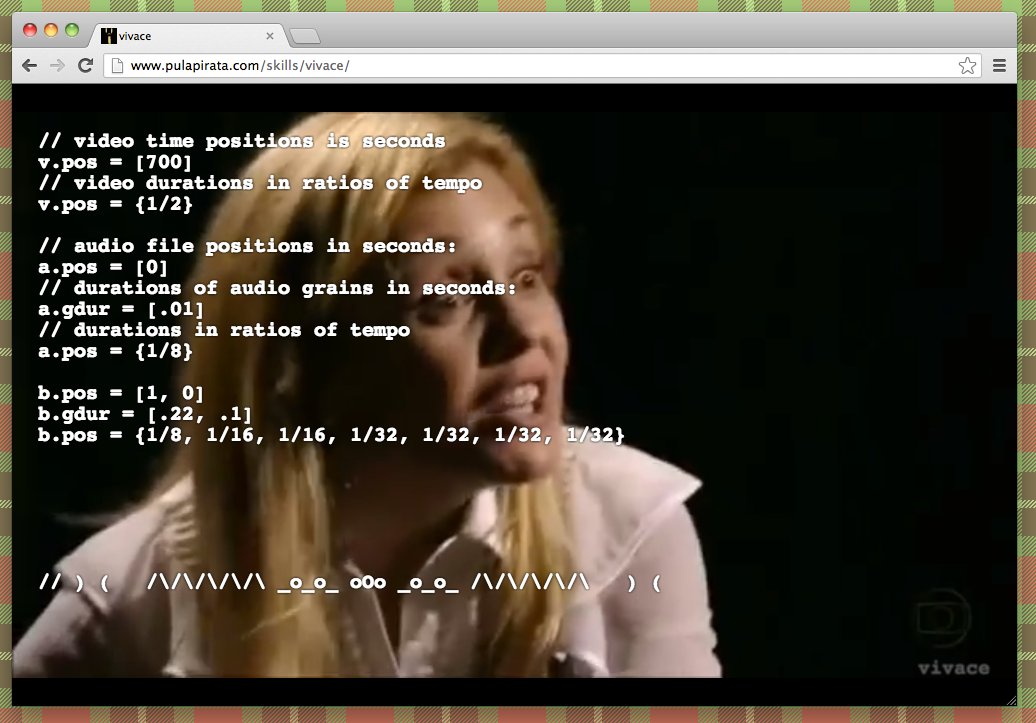
\includegraphics[scale=.3]{img/fig_novela.png}
    \caption{Videos sampled from popular Brazilian novels and B-movies
      were used as material: extreme pop-art as artifact to attract
      wider audience attention to the code.}
    \label{fig:novela}
  \end{center}
\end{figure}

All labMacambira.sourceforge.net members take part in the Brazilian
free software movement. In a way, freak coding origins should be
looked for inside this movement. It is inherent to the free software
movement the continued transmission of what is known. The same happens
on the demystification of technology and the festive and gregarious
behavior. At the performer-computer relation is where this behavior
becomes concrete. More than the materials used in the live coding
sessions, the performer's stance in relation to the computer -- as
already expressed in the described presentation -- is what really
subverts not just the highly technical computer use but the
relationship between the man and the machine. Namely a kind of a
``rock and roll'' stance. The freak coder breaks, by his own nature,
the stigma of the computer as the source of a serious and professional
posture. In the same way, breaks with the posture of the scholar
performer, stern and closed in herself. The freak coding is ``rock and
roll''. The freak coder becomes Jerry Lee of technology making
``techno-pyrophagy''. He codes and cheers at same time. The freak
coder seduces through the computer screen and by the way he codes.

\section{Conclusions and future work}

Vivace was motivated by actual performances that took place in the
recently emerging Brazilian live coding scene. The development of the
language was guided by this direct contact of performers and the wider
public. The language was designed and implemented after the
identification of common patterns already used on
presentations. Following open source practice, Vivace is being
developed by many hands from computer scientists, musicians, activists
and social scientists. At present, the language is not perfect nor
all-encompassing, but it does strike a useful balance between
flexibility and rigor, making it an interesting language for artistic
expression on collaborative sessions.

It is important to note the advantage of using the Web as the platform
for experimentation on live coding and other computer music
developments. Recent APIs like Web Audio together with the rapid
prototyping of multi-platform UI and language parsers creates a
prolific scenario. Henceforth the most interesting characteristic is
the collaboration proportioned by the Web. Using collaborative editors
we can expose an entire music program to be edited by anyone,
anywhere.

Vivace, although a ``freak coding'' language, is constrained in its
music expression. Having a domain specific language as Vivace is
interesting to express some musical ideas while others become hard or
even impossible to be expressed. In this context we assume Vivace as
one of many tools and a first step to create other languages and
collaborative systems, emerging from live coding practices. In this
way, we can tell that those performances and even Vivace are
motivating the creation of other live coding
tools. Carnaval~\footnote{Carnaval is being conceived as free software
  and a collaborative art piece since its beginning. The first
  sketches are on-line at \url{http://automata.cc/carnaval}} is one of
these new realizations, it can be seen as a ``personal TV
channel''. Each channel has a Vivace instance running on it, making
possible for anyone to remix media and create their own
composition. It is a social network of live coded remixes. Vivace,
instead of an isolated piece of software is then used as a module,
part of Carnaval.

In our experiences as performances and developers of live coding
languages we can assert this style of music realization as
inspirational and flexible. Nevertheless, we continue to search for
improvements on Vivace -- and others derived tools -- to increase the
already consolidated objective of live coding as a musical practice:
make computer music performance more human, more interactive with the
wider audience.

Future improvements are planned on Vivace: the possibility to
explicitly define large musical arcs as nested sequences related to
audio units, the use of 3D graphics APIs to render forms -- passive to
be changed by currently running audio parameters -- and text messages
to the audience, and improved UI to make the code editing more
flexible and reactive~\citep{brett}.  Along with the language and
system itself, this paper is a live initiative. Freak coding as an
artistic style will be explored more deeply on future studies --
regarding its own aesthetics -- and in already planned performances.

We want to end by underlining the importance of social aspects
regarding live coding. The authors, although working on the same
collective, were not working close to each other since the creation of
Vivace and the rise of freak coding. The performances were provided by
the union of those artists. Their union created their own tools and
influenced their own attitude. And the circle starts again.

\bibliographystyle{cmj}
\bibliography{cmjbib}
\end{document}
